The microscope is a device that performs extremely important tasks to human knowledge, in theoretical or empirical aspects. It is capable of to providing magnified views of small objects and structures. Currently, several variations of microscopes are used to investigate much smaller spaces than those visible to the naked eye \cite{wu2008microscope}. Microscopes are broadly used. In biology, areas such as physiology, histology, taxonomy, cytology and molecular biology stand out. Interdisciplinary fields such as materials sciences also apply microscopy, and health professionals use them in large scale for practical procedures, clinical analysis and research. High throughput microscopy is an important technique for the diagnosis and treatment of genetic diseases. However, to make it acceptable in the clinical environment, it is of great importance to perform high-resolution image acquisition, since low levels of sharpness can directly affect the diagnostic accuracy \cite{qiu2013evaluations}.

The advances in microscopy technologies and methods currently show a natural trend of interdisciplinary research with image processing. This bond dates back to the middle of the 20th century, when some techniques for capturing and manipulating images, primarily developed for televisions, could be
applied to microscopy images \cite{wu2008microscope}. A classic example is noise reduction, which is an important step for cryoelectronic microscopy and also for energy filtering in transmission electron microscopy, before the 3D reconstruction process on Computed Tomography scans. High noise levels hinder the necessary alignment in the reconstruction task \cite{vyas2017multiscale}.

\section{Motivation}

Biological and biomedical analysis procedures performed using microscopy images also employ image processing algorithms to obtain better results. In this sense, the concept of focus is an element of great relevance. The microscopically analyzed surfaces and structures are \emph{a priori} smooth and homogeneous to the naked eye; when magnified, these images show that those elements are irregular, i.e. they have different depths (when considering an upper view), textures and topologies. It is therefore necessary to constantly adjust the focus to get the image with the least amount of noise and lower frequency of blurred. \autoref{fig:ctenanthe_blur} illustrates the problem of differences in depth of focus in histological images of a \emph{Ctenanthe oppenheimiana} specimen with the structure of a slope, acquired in the same scene but with height settings for the objective lenses. The axial location for \autoref{fig:ctenanthe_blur}.(a) was higher than in \autoref{fig:ctenanthe_blur}.(b), and this produced clear differences among the blurred and sharp regions of both images.

\begin{figure}[ht]
    \centering
    \caption{Examples of \textit{Cthenante oppenheimiana} partially blurred images, with the leftmost (a) and rightmost parts (b) as sharp due to topological height differences.}
    \label{fig:ctenanthe_blur}
    \begin{subfigure}[t]{0.45\textwidth}
        \centering
        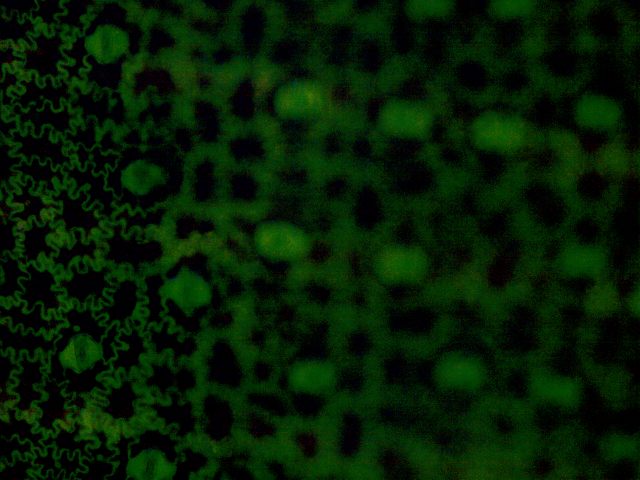
\includegraphics[scale=0.31]{images/cthenante_left.png}
        \caption{}
    \end{subfigure}%
    ~ 
    \begin{subfigure}[t]{0.45\textwidth}
        \centering
        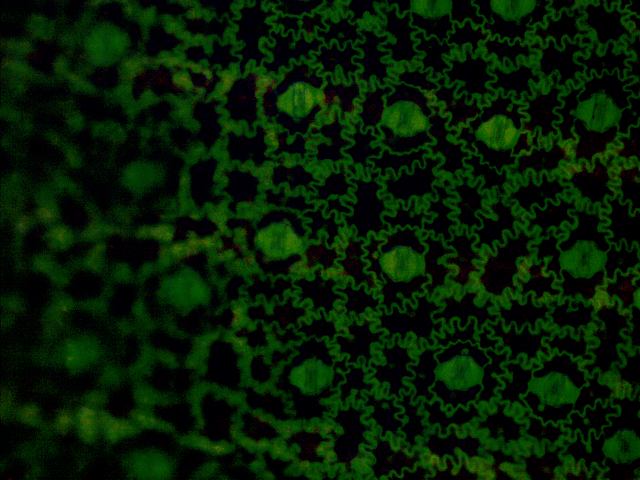
\includegraphics[scale=0.31]{images/cthenante_right.png}
        \caption{}
    \end{subfigure}
    \centering
    \fautor
\end{figure}

There are several proposed methods that address the sharpness problem in microscopy images based on image restoration techniques. According to \citeonline{ponti2016image}, the most frequently used iterative method in microscopic image restoration is the Richardson-Lucy algorithm. This is a particular case of the Maximum Likelihood Expectation Maximization algorithm with spectral extrapolation properties, which assists in the execution process at low conditions of \sigla{SNR}{Signal-to-Noise-Ratio}. Some examples presented by \cite{sun2005autofocusing} consist of
four classes: \emph{derivative algorithms}, \emph{statistical algorithms}, \emph{histogram-based algorithms} and \emph{intuitive algorithms}. Among these applications, derivative methods deserve more credit. The Fourier Transform proved itself to be
effective for low or moderate noise levels; in highly noisy environments, the resulting images were not satisfactory \cite{richardson1972bayesian}. From this evidence, probabilistic methods based on the Bayes Theorem were developed and provided images with better contrast, higher bandwidth and
edge enhancement for confocal fluorescence microscopy samples \cite{ponti2016image}.

The resulting images from such restoration processes are sharper than the original ones when validated with metrics such as the \sigla{RMSE}{Root Mean Squared Error} and the \sigla{PSNR}{Peak Signal-to-Noise-Ratio}. However, the algorithms contain limitations when it comes to degradation as input; consequently, they produce degradation as output. An alternative to restoration is to use images from the same object, with different foci, in order to obtain an enhanced depth of field image with low degradation levels.

\section{Objectives and Hyphothesis}

The objective of this work is to develop a method to perform the fusion of bright-field light microscopy images acquired indifferent focal planes. In order to achive the goal, the method will be divided into two sections, described as follows:

\begin{itemize}
    \item \emph{No-reference image quality assessment}: First, a method to quantitatively assess the quality of images based on the Fourier transform will be developed to provide an estimate of the images that may be used for fusion in a dataset, since those comprise totally out of focus images;
    
    \item \emph{Multifocus image fusion}: The sharp regions of selected images among the dataset will be fused and compose a sharp image by means of a Laplacian of Gaussian based method.
    
\end{itemize}

It is hypothesized that frequency domain information from images may be used to quantify sharpness of bright-field microscopy images. Simultaneously, we also have the hypothesis that image fusion methods that employ edge detection by means of the Laplacian operator and its derivatives, e.g. the Laplacian of Gaussian, perform well on bright-field images. 

\section{Publications}

\begin{itemize}
    \item Waiting...
    
    \item \cite{catanante2020frequency} Victor Augusto Alves Catanante, Odemir Martinez Bruno, and João do Espírito Santo Batista Neto. ``Frequency domain kurtosis-based no-reference image quality assessment for bright-field microscopy images''. \textbf{To be submitted}.
\end{itemize}

\section*{Structure of the document}

This monograph is organized as follows:

\begin{itemize}
    \item \autoref{chapter:fundamentals-of-optics-and-light-microscopy} provides several essential concepts of Optics for the understanding of Light Microscopy in general and, particularly, the Bright-field Microscopy;
    
    \item \autoref{chapter:blur-characterization-and-image-formation} comprises relevant information about the bright-field microscopy image formation process and also describes the defocus blur property;
    
    \item \autoref{chapter:theoretical-background} provides the theoretical basis of this work, i.e. image transforms, enhancement, registration, fusion and quality assessment, as well as theories from statistics to analyze the data;
    
    \item \autoref{chapter:related-work} performs a literature review on no-reference image quality assessment, multifocus image fusion and consequently presents the literature that motivated the development of our method;
    
    \item \autoref{chapter:materials-and-methods} exposes details of both of our methods and also presents our proposed image datasets;
    
    \item \autoref{chapter:results} presents our results with the proposed datasets and exposes a discussion concerning the quantitative and qualitative analysis of them;
    
    \item \autoref{chapter:conclusions} summarizes everything that was achieved, as well as information to guide future work on the field and improvements in the methods;
    
    \item \autoref{chapter:definitions-and-proofs} is the result of mathematical reasoning to prove some properties concerning the method which were hypothesized true.
    
\end{itemize}
